\section{Systematics}
\label{sec:systematics}
Systematics associated with event reconstruction, the mixing parameters,
and trigger efficiency are considered for this analysis.
The event reconstruction systematics are uncertainties on the energy reconstruction
scale and resolution, position reconstruction resolution and scale, and the
resolution of the direction reconstruction.
The position and energy systematics must be known to assess uncertainties
on the efficiencies for the fiducial volume cut and for what fraction
of solar neutrino interactions will fall into each energy bin.
Since the solar event rate is extracted from a fit to the angular distribution
of events with respect to the solar direction, it's important that the
detector's angular resolution be well constrained.
The uncertainties for these reconstructed quantities are determined from
analysis of $\ce{^{16}N}$ data.
All systematics are treated in the same, or a similar, way, to propagate
their effect to the flux result.
First the systematic uncertainty on a reconstructed quantity (\textit{e.g.} energy, position etc.)
is determined from an analysis of the $\ce{^{16}N}$ data.
Then, the relevant reconstructed Monte Carlo quantity 
is modified according to the one-sigma systematic uncertainty.
From this A 2D histogram in energy and $\cos\theta_{sun}$ is produced using the
modified event quantities, applying the standard cuts.
Finally, the flux result is found by performing a fit to data using the systematically
adjusted histogram as input.
The difference between the best fit value found using unmodified event quantities
and using the modified quantities is taken to be the one-sigma systematic uncertainty.
How each variable is modified, and any deviations from this process of propagating systematics is detailed below.
All systematics are treated as uncorrelated; variables are modified according to
only one systematic at a time.

\subsection{Energy Systematics}
The detector resolution $\sigma_{E}$ and relative energy scale $\delta_{E}$ are determined
from the $\ce{^{16}N}$ detected energy spectrum.
The detected energy spectrum is modeled by $P(T_\mathrm{e})$ in electron equivalent
energy, and is given by $P_{\mathrm{source}}(T_{\mathrm{e}})$
convolved with a normalized Gaussian distribution.
\begin{equation}
    P(T_\mathrm{e}) = N \int P_\mathrm{source}(T^{\prime}_{e})\frac{1}{\sqrt{2\pi}\sigma_{E}}e^-{\frac{\left((1+\delta_E)T_\mathrm{e}-T^{\prime}_{e}\right)^{2}}{2\sigma^{2}_{E}}}dT^{\prime}_{e}\text{.}%-\Delta E
\label{eq:convolution}
\end{equation}
$P_\mathrm{source}(T_{\mathrm{e}})$ represents the distribution of deposited energy in
the detector from the $\ce{^{16}N}$ source.
Since the $\ce{^{16}N}$ emits gammas into the detector the mapping between
gamma energy and electron equivalent energy is done by finding the electron
energy that can produce the same number of Cherenkov photons
as each gamma; this is not a one-to-one mapping because the same electron or gamma
energy will not always produce the same number of photons.
The mapping is determined from simulation and is shown in
Fig.~\ref{fig:cherenkov_energy_map}.
The gamma to electron energy mapping is then applied to the simulated $\ce{^{16}N}$
gamma energy spectrum to determine $P_\mathrm{source}(T_{\mathrm{e}})$.

\begin{figure}[htbp]
\centering
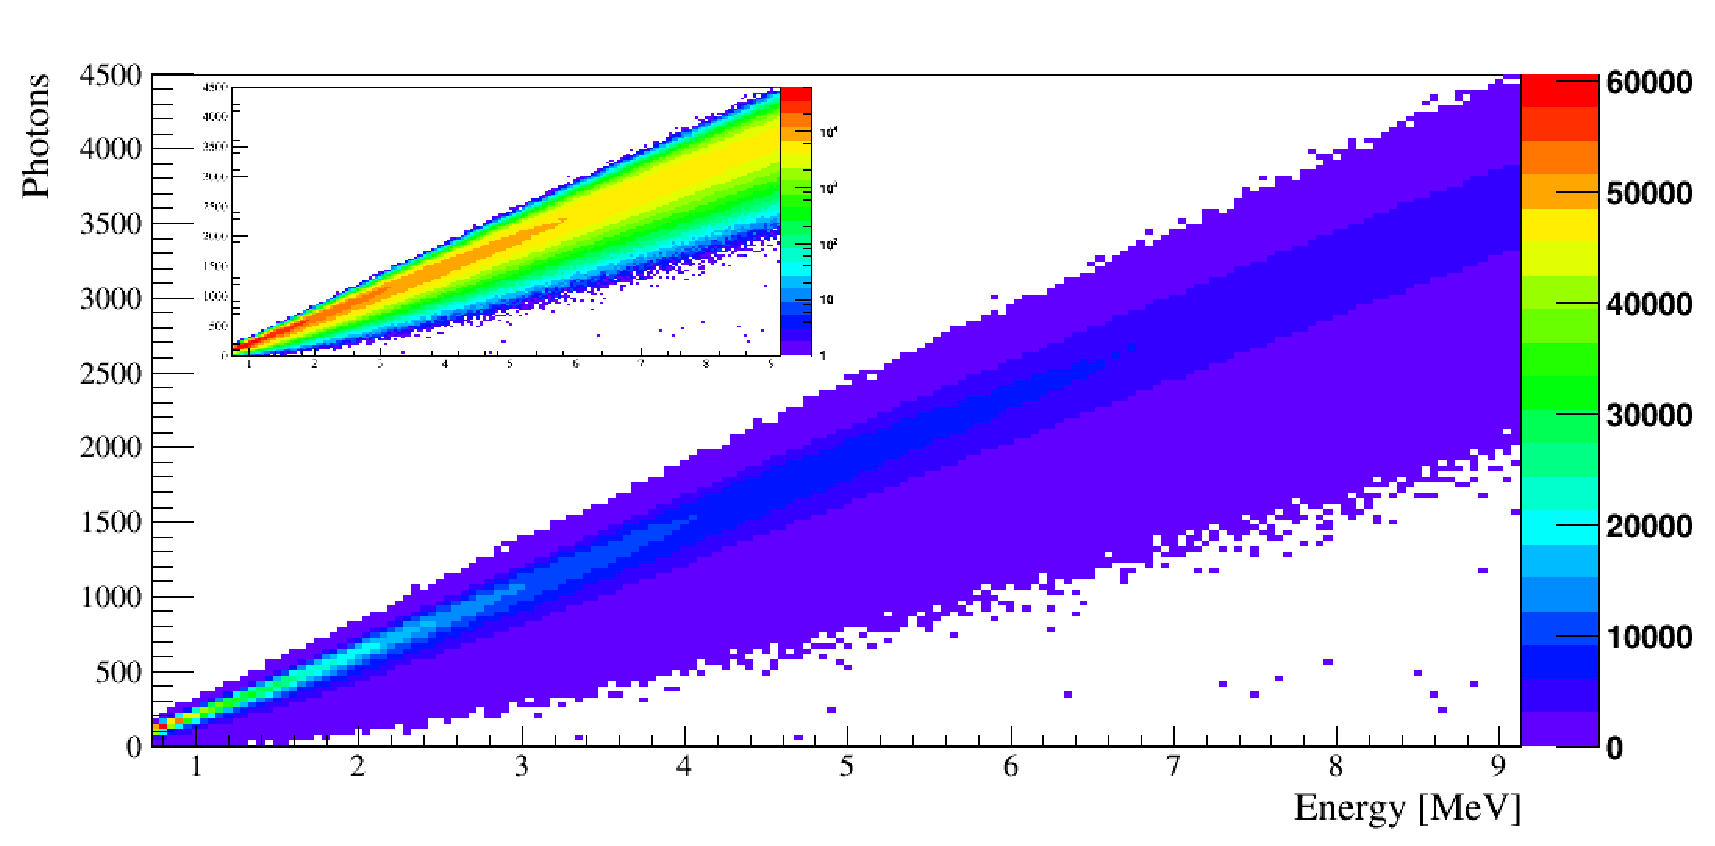
\includegraphics[width=0.78\textwidth]{cherenkov_nhit_energy_map.eps}
\caption[Electron Cherenkov Photon Product PDF]{ The map between electron
energy and expected Cherenkov photons production.  Used for the energy
calibration to map between gamma energy and equivalent electron energy.  This is
the same PDF used by EnergyRSP to estimate energy from the observed PMT hits.}
\label{fig:cherenkov_energy_map}
\end{figure}

\begin{figure}[htbp]
\centering
\begin{subfigure}{0.48\textwidth}
\centering
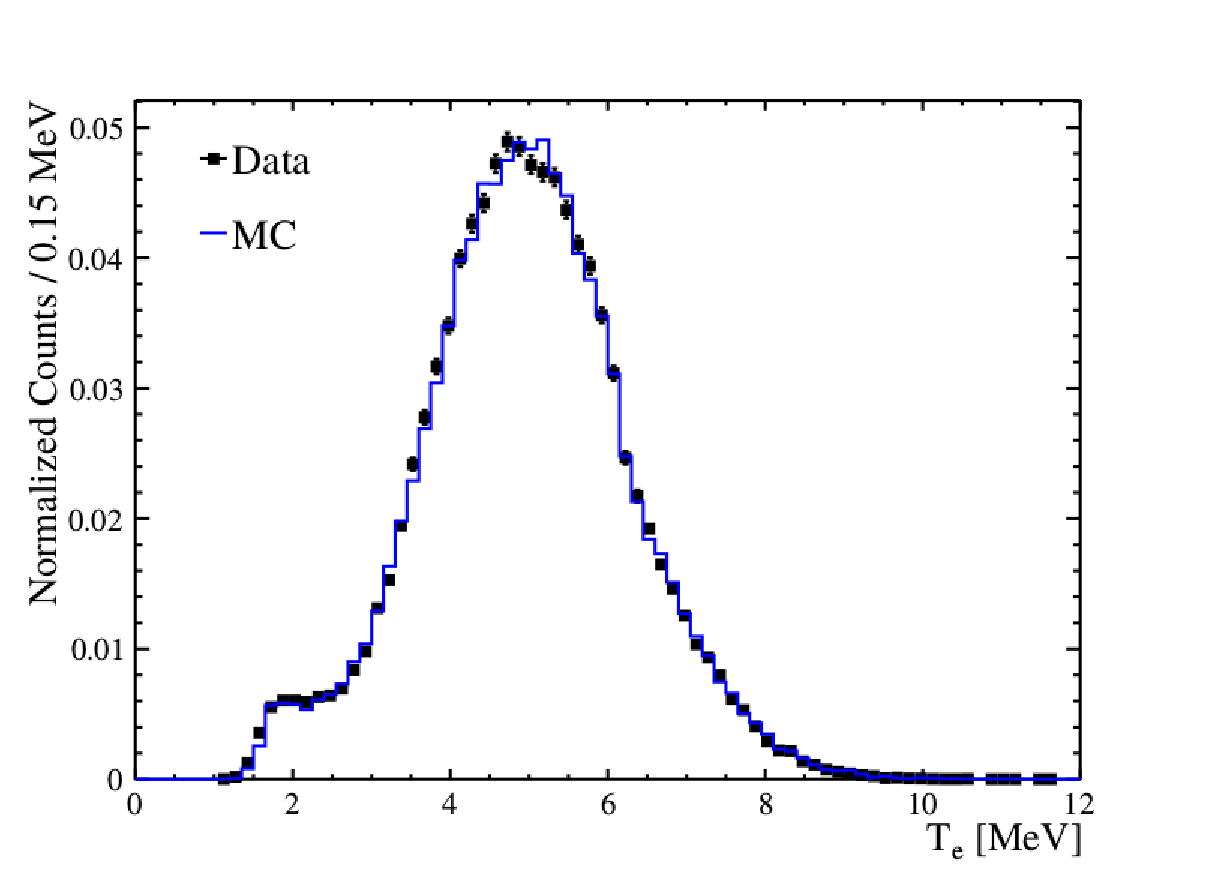
\includegraphics[width=\textwidth]{energy_data_vs_mc}
\caption[]{}
\end{subfigure}
\hfill
\begin{subfigure}{0.48\textwidth}
\centering
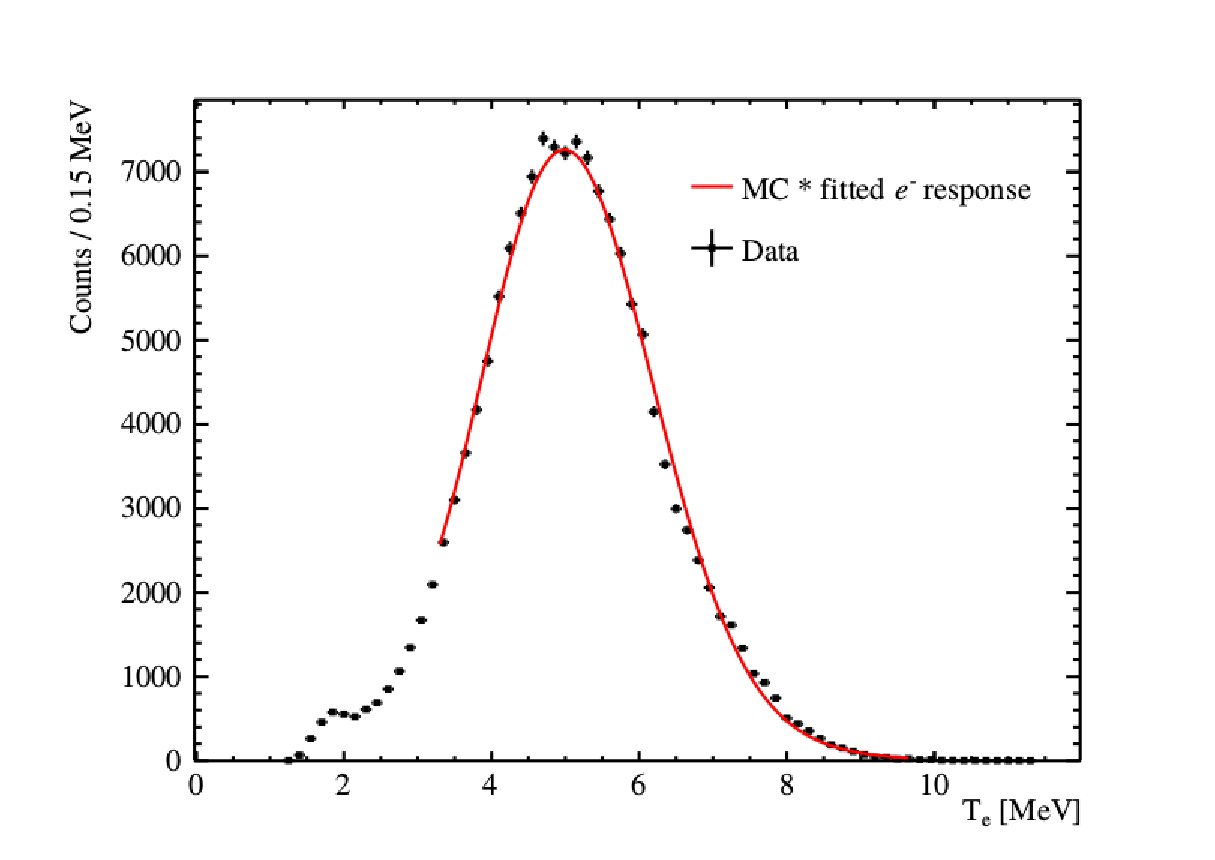
\includegraphics[width=\textwidth]{N16energyFit}
\caption[]{}
\end{subfigure}
\caption[$\ce{^{16}N}$ Energy Comparisons]{ (a) The comparison between
reconstructed energy for $\ce{^{16}N}$ data and Monte Carlo.  (b) Fit of
Eqn.~\eqref{eq:convolution} to distribution of reconstructed energies for
detected central $\ce{^{16}N}$ events.}
\label{fig:n16_energy}
\end{figure}
The values for $\sigma_{E}$ and $\delta_{E}$ are extracted from~\eqref{eq:convolution}
by performing a fit to the reconstructed $\ce{^{16}N}$ energy spectrum.
The fit is done to both simulated $\ce{^{16}N}$ data and to detector data,
each determining their own values for $\sigma_{E}$ and $\delta_{E}$.
As is show in Fig~\ref{fig:n16_energy}, this fit is only performed
over the energy range $3.25$ to $9.6$\,MeV, at energies outside this range
difficult to model source-container effects dominate the energy spectrum.
It's worth noting that $\sigma_{E}$ represents only the resolution provided by detector
effects, resolution from effects such as photon statistics are accounted
for in $P_\mathrm{source}(T_{\mathrm{e}})$.

Values for $\sigma_{E}$ and $\delta_{E}$ are extracted for data taken, or simulated, with
the $\ce{^{16}N}$ source at many position, allowing for a position dependent
determination of the energy scale and resolution.
Fitting to both simulated and to detected data allows for a correction to
be created that can make the two datasets match better, however the data
used to create the correction cannot then be used to determine systematics.
So the $\ce{^{16}N}$ data was split into two datasets, one for determining
what correction should be applied to simulation, the other for evaluating
the remaining uncertainties after the correction is applied.

The data for the correction is further divided into position bins in $z$ and
$\rho$, where $\rho = \sqrt{x^{2} + y^{2}}$. The choice of binning is motivated
by the symmetry of the detector, the detector is very symmetric for an interchange
of $x$ and $y$ or $x,y \rightarrow -x,-y$.
There exists, however, significant asymmetries along the $z$ axis
from the detector neck and from the rope-net along the top of the AV\@.
The data is divided into 4-bins along the $\rho$ direction each $200$\,cm long
and bins of $57$\,cm height along the $z$ axis. The number of bins along the
z-axis varies for each slice in $\rho$ because data was primarily taken within
the AV.\@
Figure~\ref{fig:n16_uniformity} shows position dependence of the fits for
$\delta_{E}$ and $\sigma_{E}$ in each bin for both simulated and detected
events.

\begin{figure}[htbp]
\centering
\begin{subfigure}{0.49\textwidth}
\centering
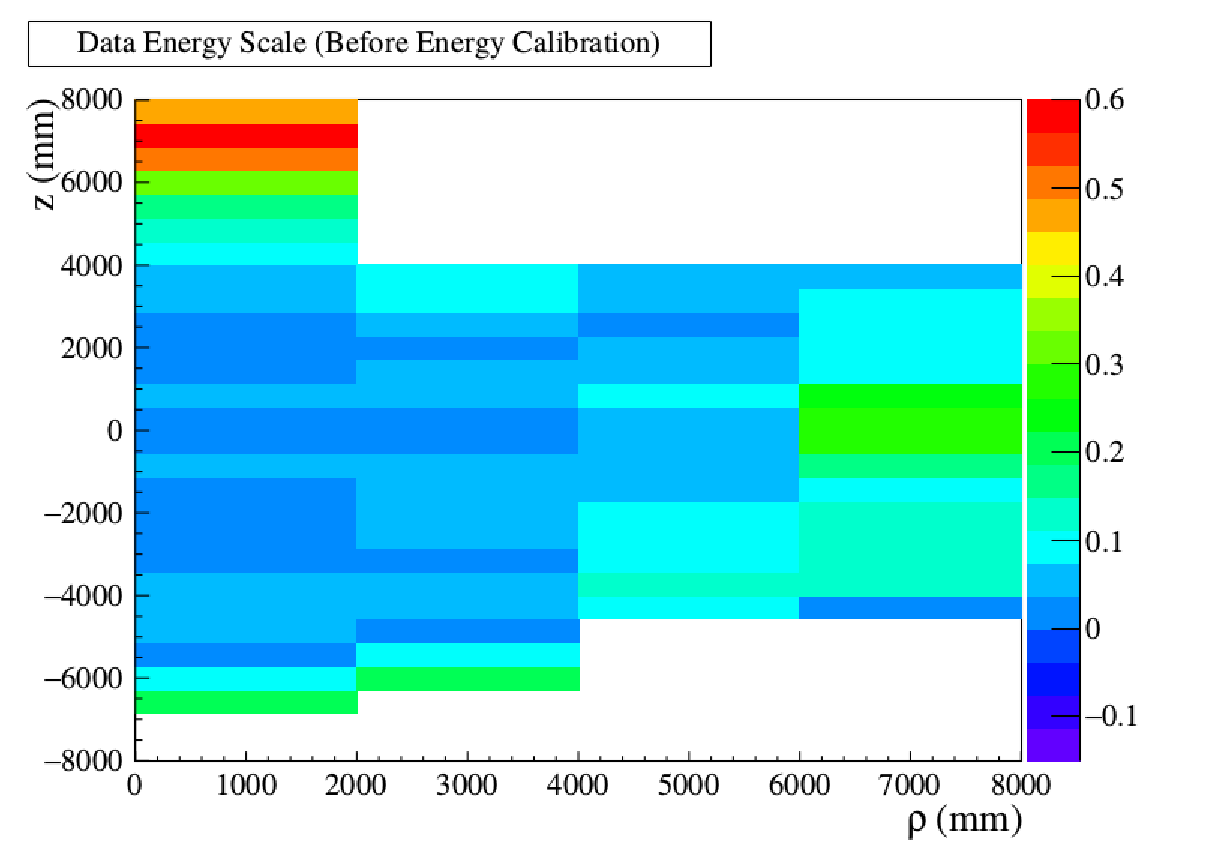
\includegraphics[width=\textwidth]{data_scale_uniformity}
\caption[]{}
\end{subfigure}
\hfill
\begin{subfigure}{0.49\textwidth}
\centering
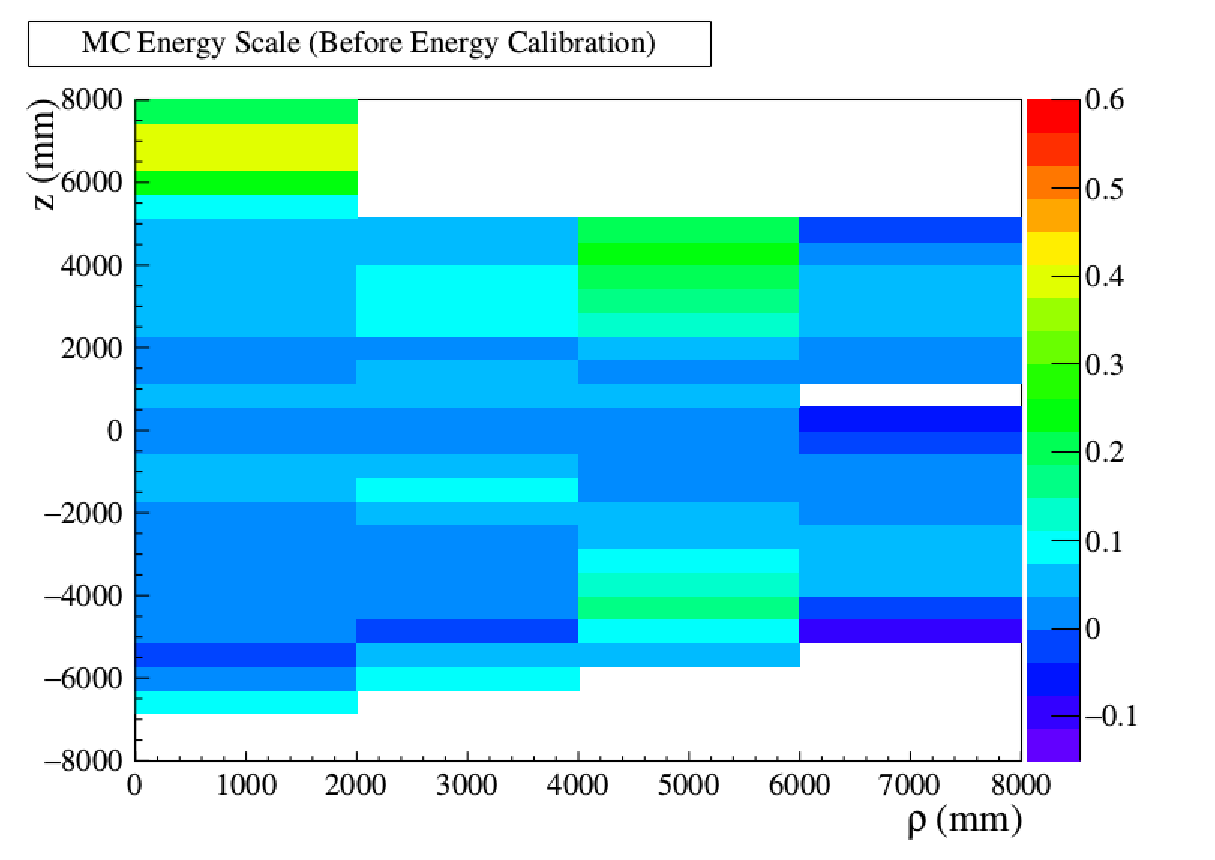
\includegraphics[width=\textwidth]{mc_scale_uniformity}
\caption[]{}
\end{subfigure}

\begin{subfigure}{0.49\textwidth}
\centering
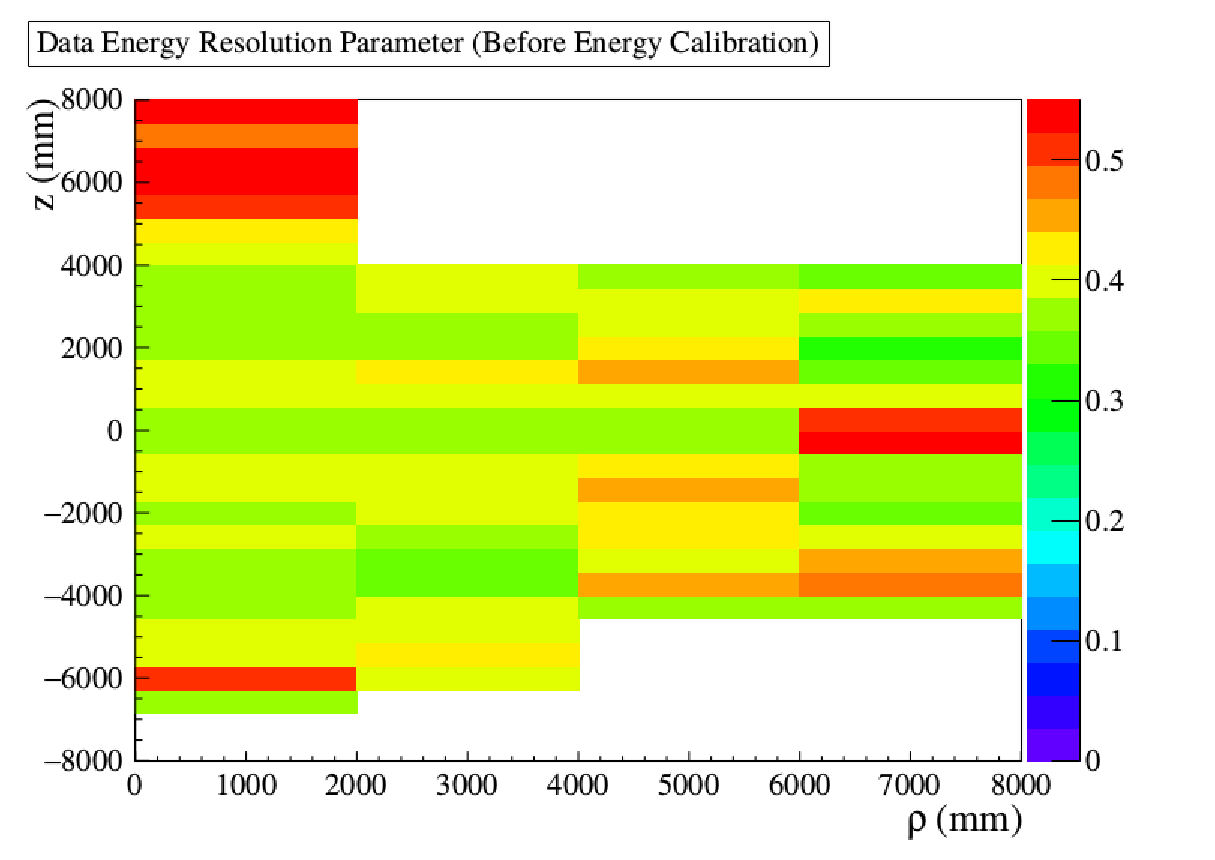
\includegraphics[width=\textwidth]{data_sig_uniformity}
\caption[]{}
\end{subfigure}
\hfill
\begin{subfigure}{0.49\textwidth}
\centering
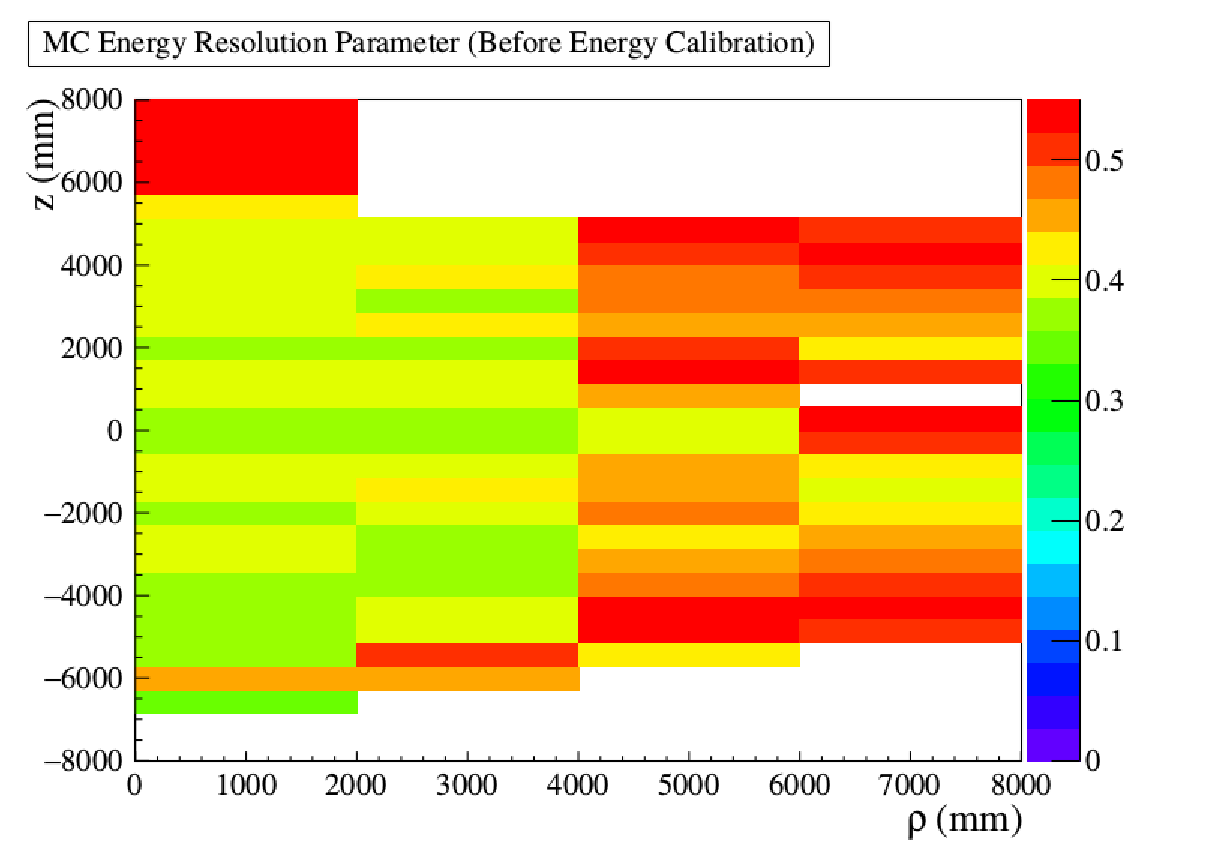
\includegraphics[width=\textwidth]{mc_sig_uniformity}
\caption[]{}
\end{subfigure}
\caption[Position Depedence of Energy Scale and Resolution from $\ce{^{16}N}$]
{The best fit energy scale before for detected (a) and Monte Carlo simulated (b)  $\ce{^{16}N}$
events as a function of position.
And the best fit energy resolution parameter for detected (c) and 
simulated (d) $\ce{^{16}N}$ events}
\label{fig:n16_uniformity}
\end{figure}

\begin{figure}[htbp]
\begin{subfigure}{0.49\textwidth}
\centering
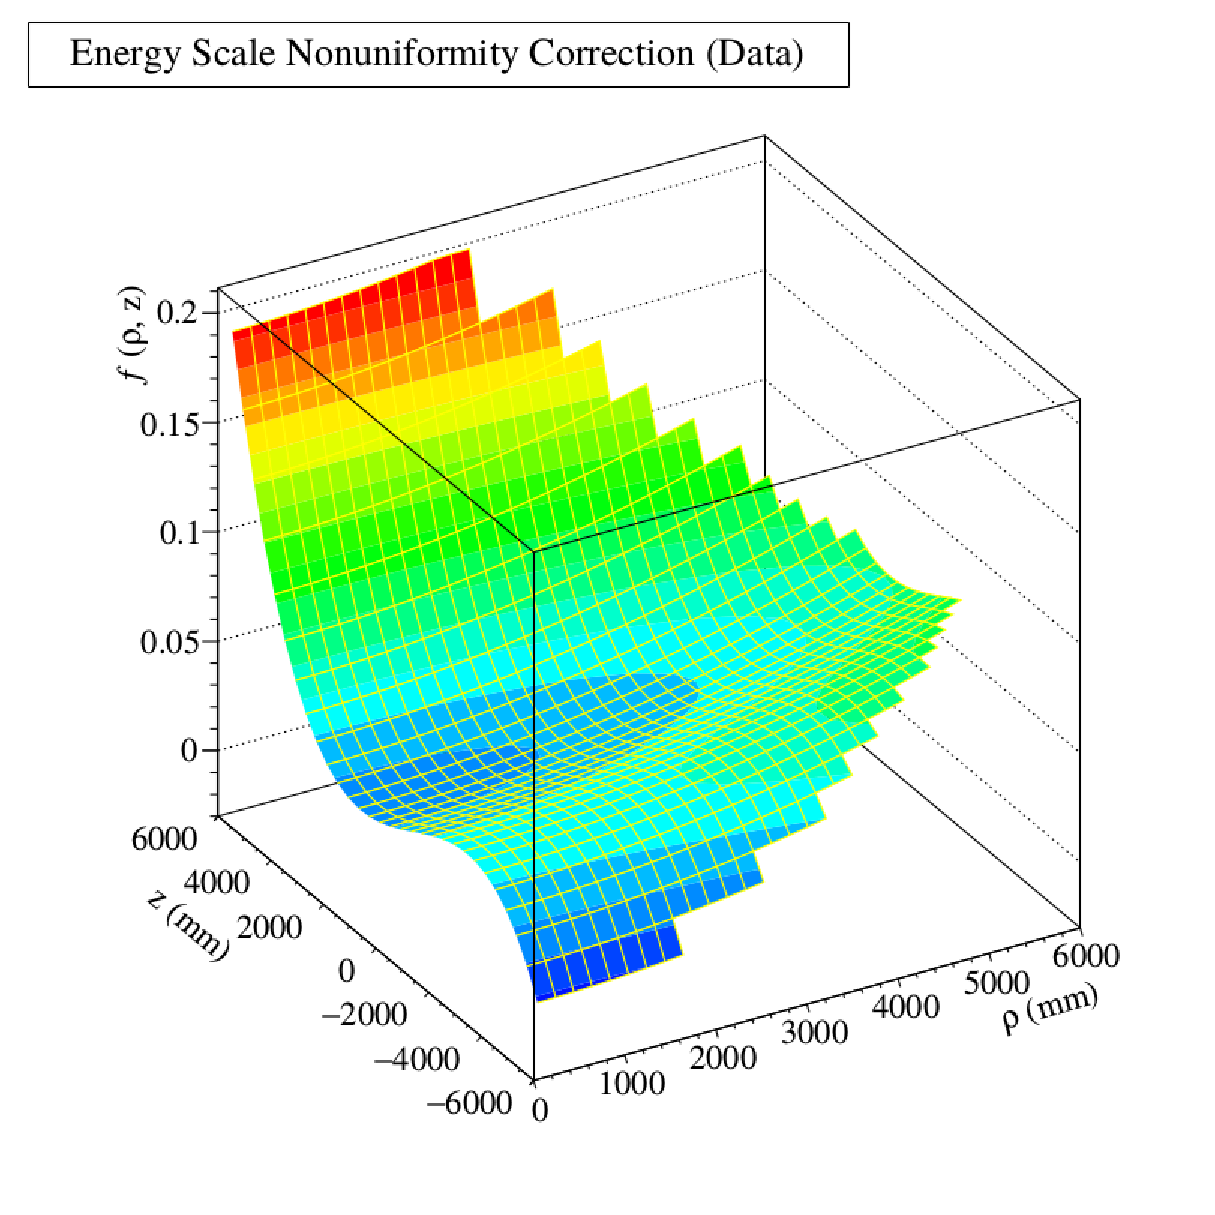
\includegraphics[width=\textwidth]{energy_uniformity_correction}
\caption[]{}
\end{subfigure}
\hfill
\begin{subfigure}{0.49\textwidth}
\centering
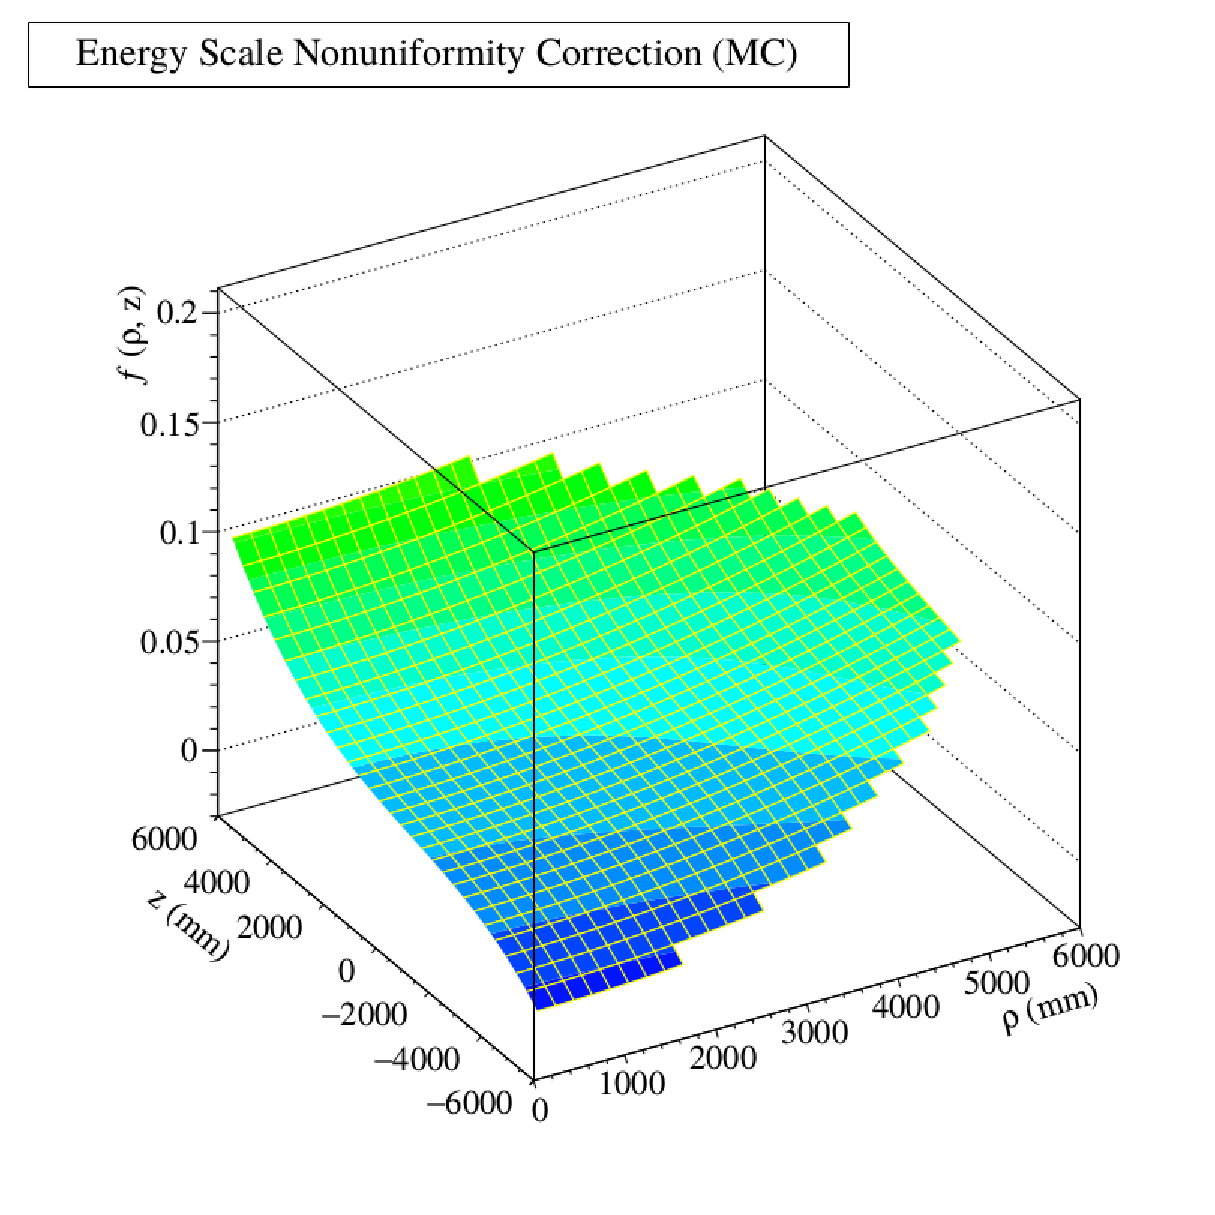
\includegraphics[width=\textwidth]{energy_mc_uniformity_correction}
\caption[]{}
\end{subfigure}

\begin{subfigure}{0.49\textwidth}
\centering
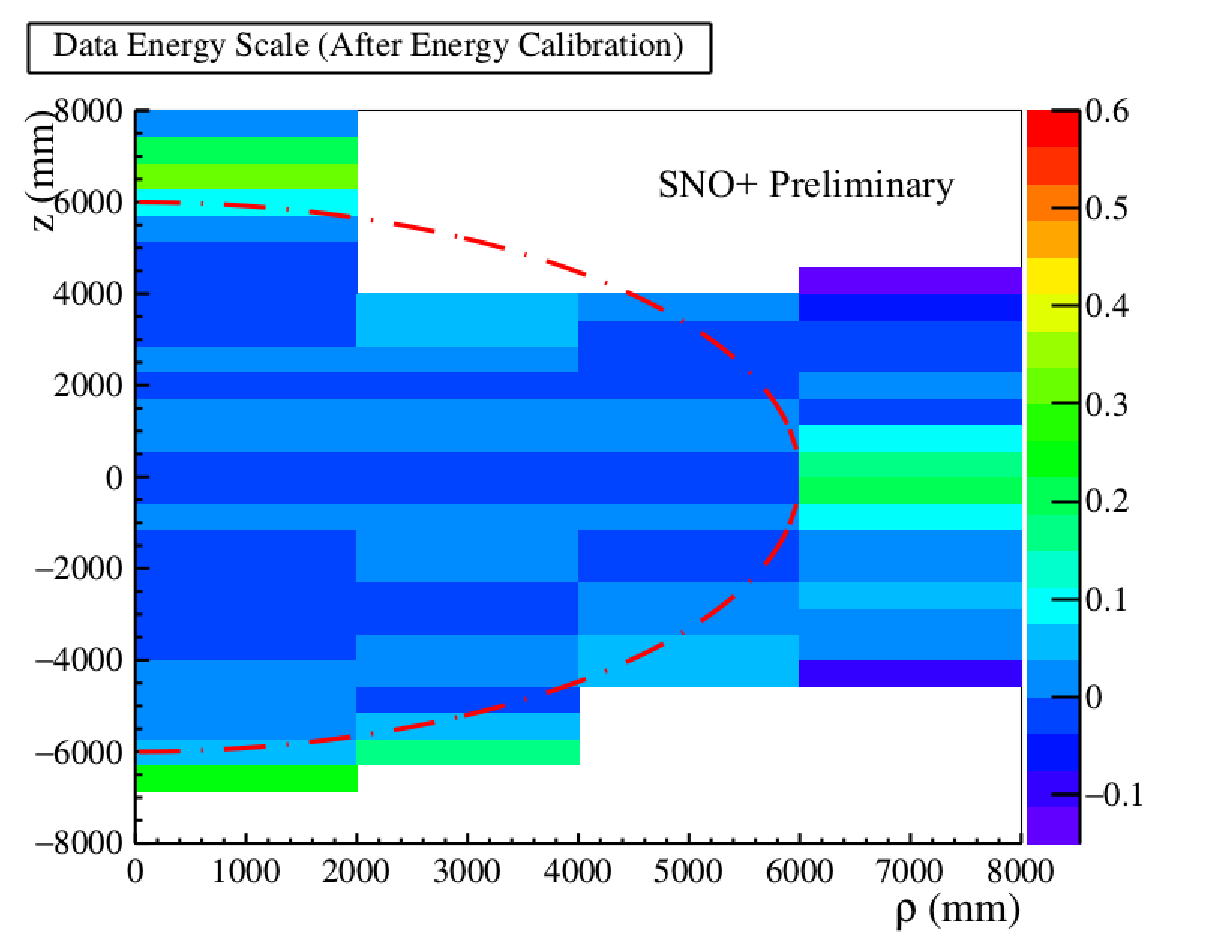
\includegraphics[width=\textwidth]{Res_data}
\caption[]{}
\end{subfigure}
\hfill
\begin{subfigure}{0.49\textwidth}
\centering
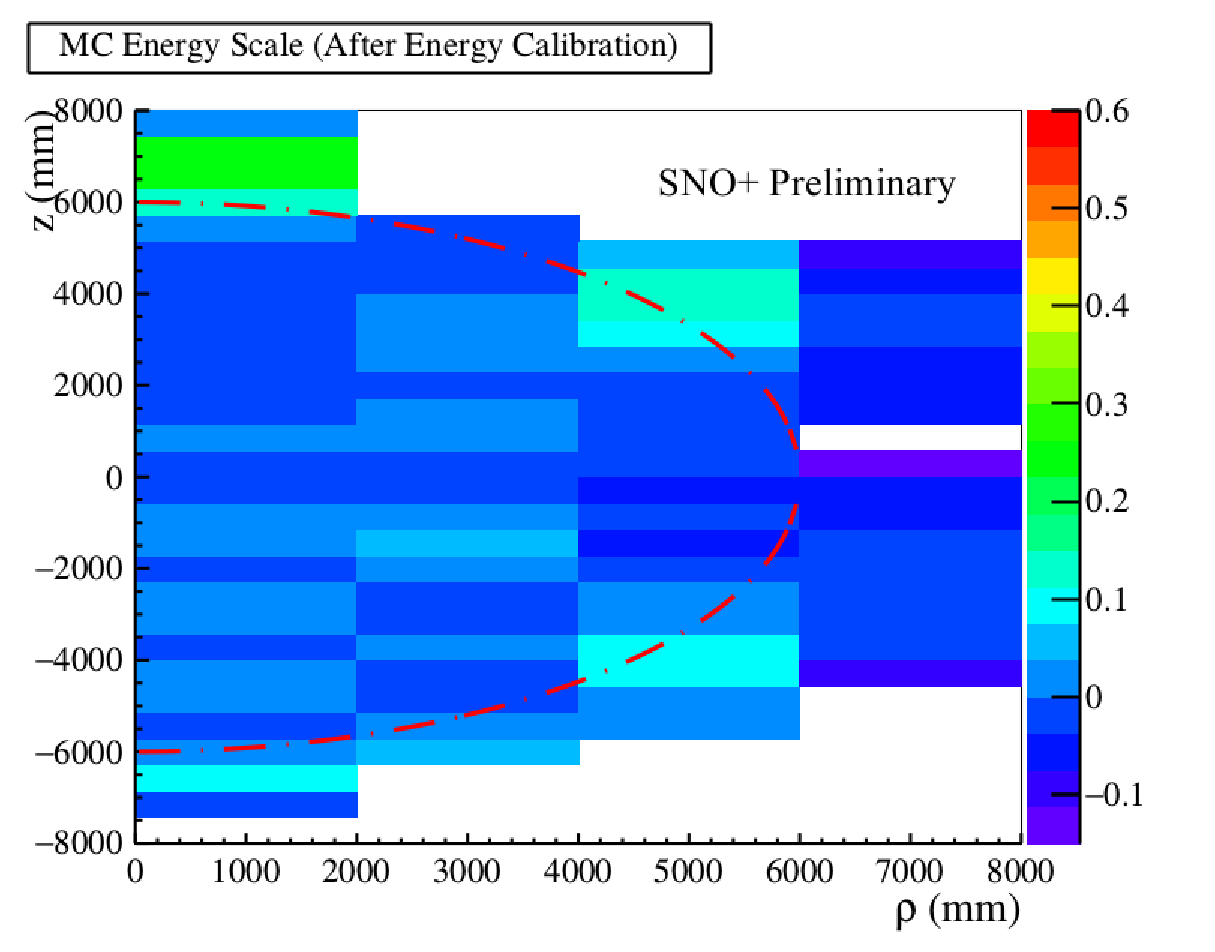
\includegraphics[width=\textwidth]{Res_MC}
\caption[]{}
\end{subfigure}
\caption[Energy Scale Uniformity Correction and Results]{The energy scale
non-uniformity correction for data (a) and MC simulation (b).
The measured energy scale as a function of position after the application
of the non-uniformity correction for data (c) and MC simulation (d).}
\label{fig:uniformity_corrections}
\end{figure}

Variations in $\delta_{E}$ along $z$ and $\rho$ were modeled by a polynomial given by,
\begin{equation}
    \delta_{E}(\rho^{2}, z) = A + \left[(1+B\rho^{2})(1+Cz+Dz^{2}+Ez^{3}) - 1\right]\text{.}
    \label{eqn:escale_position_dependence}
\end{equation}
Values for $A$, $B$, $C$, $D$, and $E$ are extracted from a fit to the observed
spatial variation of $\delta_{E}$ for simulation and data and are given in
table~\ref{tbl:n16_position_escale}.
The reconstructed energies of simulated and detected 
events are then corrected according to~\eqref{eqn:escale_position_dependence} by
their respective best fit values.
Figure~\ref{fig:uniformity_corrections} shows the correction as a function of
position in the detector and the energy scale measured across the detector
after the application of the correction.
The energy resolution is evaluated as a function of position but no correction
is determined from it.
\begin{table}
    \centering
\begin{tabular}{|c | c | c | c |c|c|}
\hline
& A&B&C&D&E\\
\hline
Data& 2.53e-2& 1.48e-9 & -5.44e-6 & 2.14e-9 & 6.49e-13\\
Simulation& 3.33e-2& 9.48e-10& 3.77e-6& 4.46e-10& 1.43e-13\\
\hline
\end{tabular}
\caption{Best fit values for~\eqref{eqn:escale_position_dependence} for
simulated and detected data, determined using units of mm for $z$ and $\rho$.}
\label{tbl:n16_position_escale}
\end{table}

After the correction is applied to remaining half of the calibration dataset
$\sigma_{E}$ and $\delta_{E}$ are determined once more as a function of position.
The bin-by-bin differences in $\sigma_{E}$ and $\delta_{E}$ between
simulated and detected data are taken as the systematic uncertainty for those
parameters, with additional fit uncertainties added in quadrature.
Averaging the bin-by-bin systematic uncertainty over the detector volume relevant
for the solar analysis yields a remaining uncertainty on the energy
scale of $\delta_{E} =1 \pm 2.0\%$ and
$\delta_{\sigma} = +0.018\text{, }-0.016$ to be the uncertainty on
the energy resolution.

To create the systematically modified energy resolution histograms for the
solar analysis the reconstructed
energy of each MC simulated event is mapped to a normalized Gaussian distribution with a
mean value of the event's energy and a
variance given by
\begin{equation}
  \sigma^{2} = \sigma_{E}^{2}\left(\left(1 + \delta_{\sigma}\right)^2 - 1\right)\text{.}
  \label{eqn:systmatic_esmear}
\end{equation}
This process of mapping a single energy value to a Gaussian distribution is
referred to as ``smearing''.
Here $\sigma_{E}$ is given by $\sqrt{E}$ to match the functional form used in
Eqn~\ref{eq:convolution}.
The idea behind this smearing is to compensate for the possibility that our
Monte Carlo simulation could have a systematically smaller energy resolution
than occurs in real data.
So by applying a smearing the Monte Carlo energy resolution is artificially
deteriorated, and the uncertainty on the resolution is accounted for.
A similar process does not exist to account for the possibility that the
MC simulation has a poorer energy resolution than data taken from the
real detector; there's no way to ``un-smear'' the reconstructed MC event
energy.
To account the effect of an over-estimated energy resolution the error on
the result is assumed to be symmetric.
As a penalty for this assumption the larger uncertainty between the positive
and negative uncertainty on the energy resolution is used.
For each event, and for each energy bin of the systematically modified histogram
is fill by an amount equal to the integral of the event's Gaussian across that
energy bin.
The Gaussian generated from each event is integrated across each energy bin.

Systematically varied histograms for the energy scale is generated by simply
modifying the reconstructed kinetic energy of each event according to
\begin{equation}
  T^{\prime}_{e} = \delta_{E}T_{e}\text{.}
\end{equation}
This leads to a straightforward shift of $\pm 2.0\%$ for all energies.
At all points in the analysis afterwards $T^{\prime}_{e}$ is used instead of $T_{e}$
and the systematic histogram is generated the same way the standard analysis histograms
are.

\subsection{Fiducial Volume}
Uncertainty on the fiducial volume comes from systematics associated
with the position reconstruction.
If the position reconstruction is more likely to pull an event towards the
middle of the detector in MC simulation than in data, it will result in an over
prediction of the number of events that will pass the FV cut.
This possibility is accounted for by shifting the reconstructed position of
simulated events according to the uncertainty, the fiducial volume cut is
applied to those shifted positions.
Shifting the events results in modified PDFs, those PDFs are used in the fit
for the solar event rate, the difference between the best fit value extracted
with the modified PDFs and the best fit value from the standard PDFs is taken
to be the systematic uncertainty.

The systematic uncertainty on position reconstruction is evaluated
using $\ce{^{16}N}$ data and simulation.
The difference between the source position and the reconstructed
position of each event is determined and histogrammed.
A fit to that distribution is performed using a model of a Gaussian distribution
with exponential tails convolved with a distribution for the first gamma interaction
distance. The equation for this is given by,
\begin{equation}
    P(x)  = A \cdot \bigg[ \bigg(\frac{1 - \alpha}{\sqrt{2\pi}\sigma}e^{- \frac{(x-\mu)^2}{2\sigma^2}} + \frac{\alpha }{2 \tau}e^{-\frac{|x-\mu|}{\tau}}\bigg) \circledast P_{\gamma}(x) \bigg]\text{.}
    \label{eqn:n16_position_model}
\end{equation}
Where $\mu$ and $\sigma$ are respectively the center and width of the Gaussian,
$\tau$ represents the decay rate for the exponential tails, and $\alpha$ represents
the relative strength of the exponential~vs.~the Gaussian;
$P_{\gamma}(x)$ is distribution of distance travelled by an $\ce{^{16}N}$
gamma before it's first interaction, it is determined from a separate MC
simulation.
Finally, $A$ is an overall normalization to account for the number of events
included in the distribution.
The Gaussian and exponential portion of
\eqref{eqn:n16_position_model} represents the spread introduced by the detector
and position reconstruction, the $P_\gamma$ term represents the intrinsic spread
in interaction positions from the source itself.
The distribution used for $P_\gamma$ in show in Fig~\ref{fig:gamma_first}
Figure~\ref{fig:n16_position_comparison} shows a comparison between data
and Monte Carlo simulation for reconstructed position and an example fit to the data
for a central $\ce{^{16}N}$ dataset.
\begin{figure}[htbp]
    \centering
    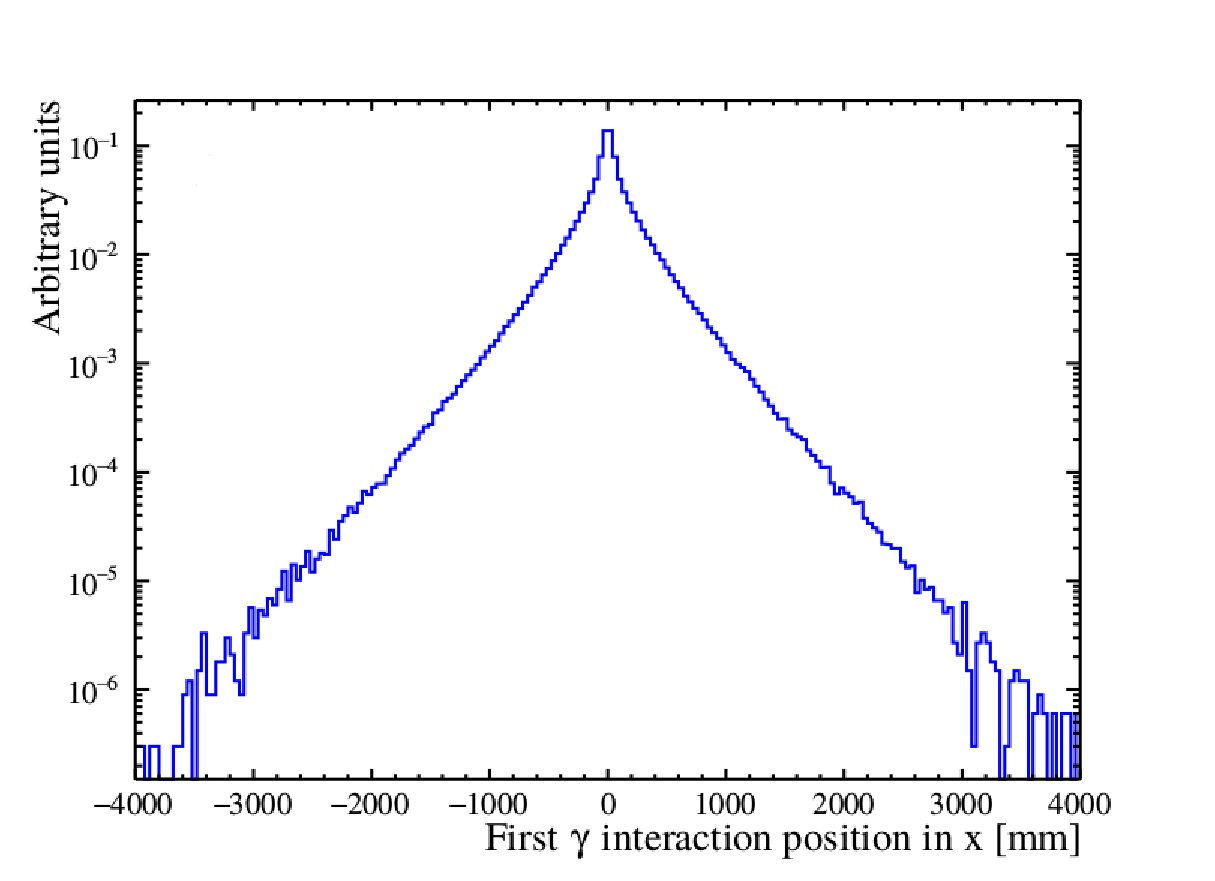
\includegraphics[width=0.69\textwidth]{gamma_first_scattering}
    \caption[Distribution of Gamma First Interaction Distance]{
    The distribution of first interaction distances for gamma ray produced
    in the $\ce{^{16}N}$ source. Produced from MC simulation and used in
    Eqn.~\eqref{eqn:n16_position_model}.}
    \label{fig:gamma_first}
\end{figure}

\begin{figure}[htbp]
\centering
    \begin{subfigure}{0.49\textwidth}
        \centering
        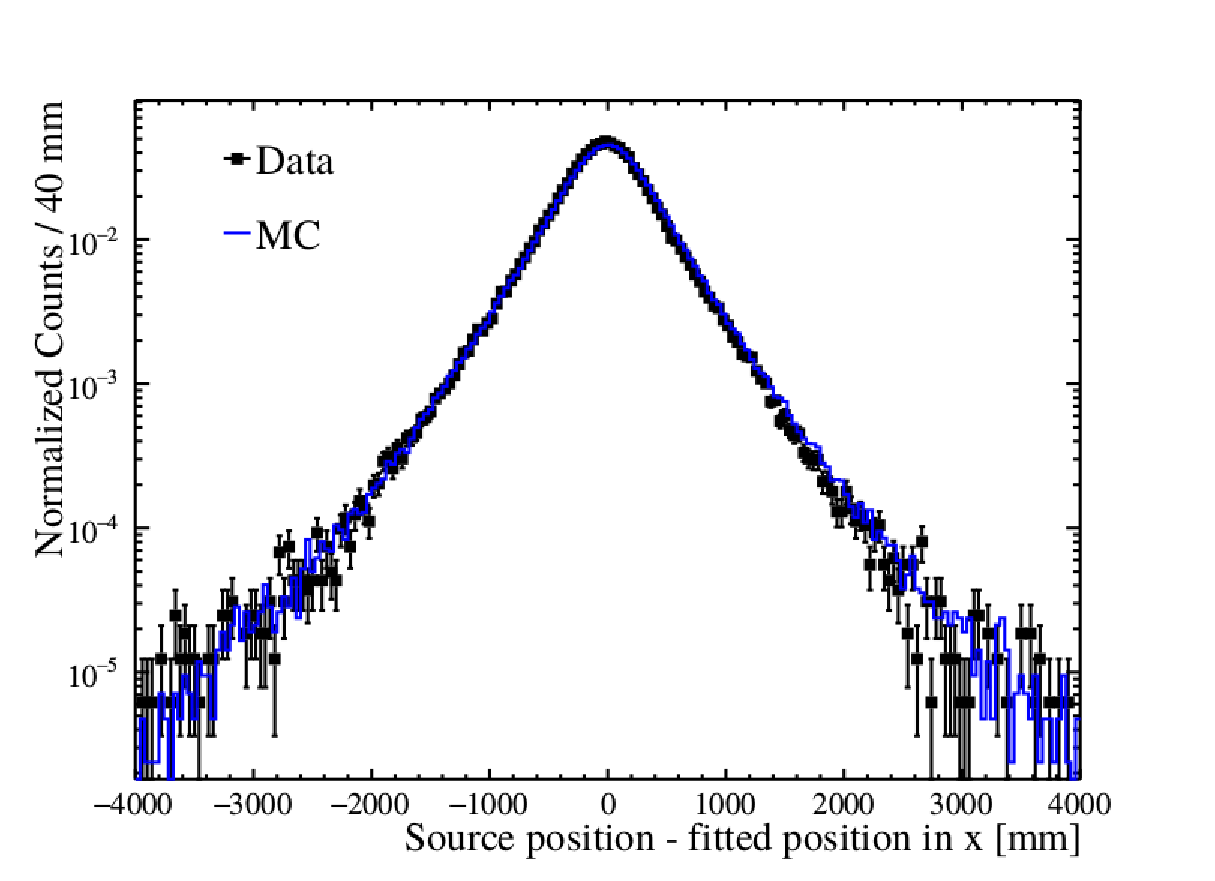
\includegraphics[width=\textwidth]{Position_data_vs_mc}
        \caption{}
    \end{subfigure}
    \begin{subfigure}{0.49\textwidth}
        \centering
        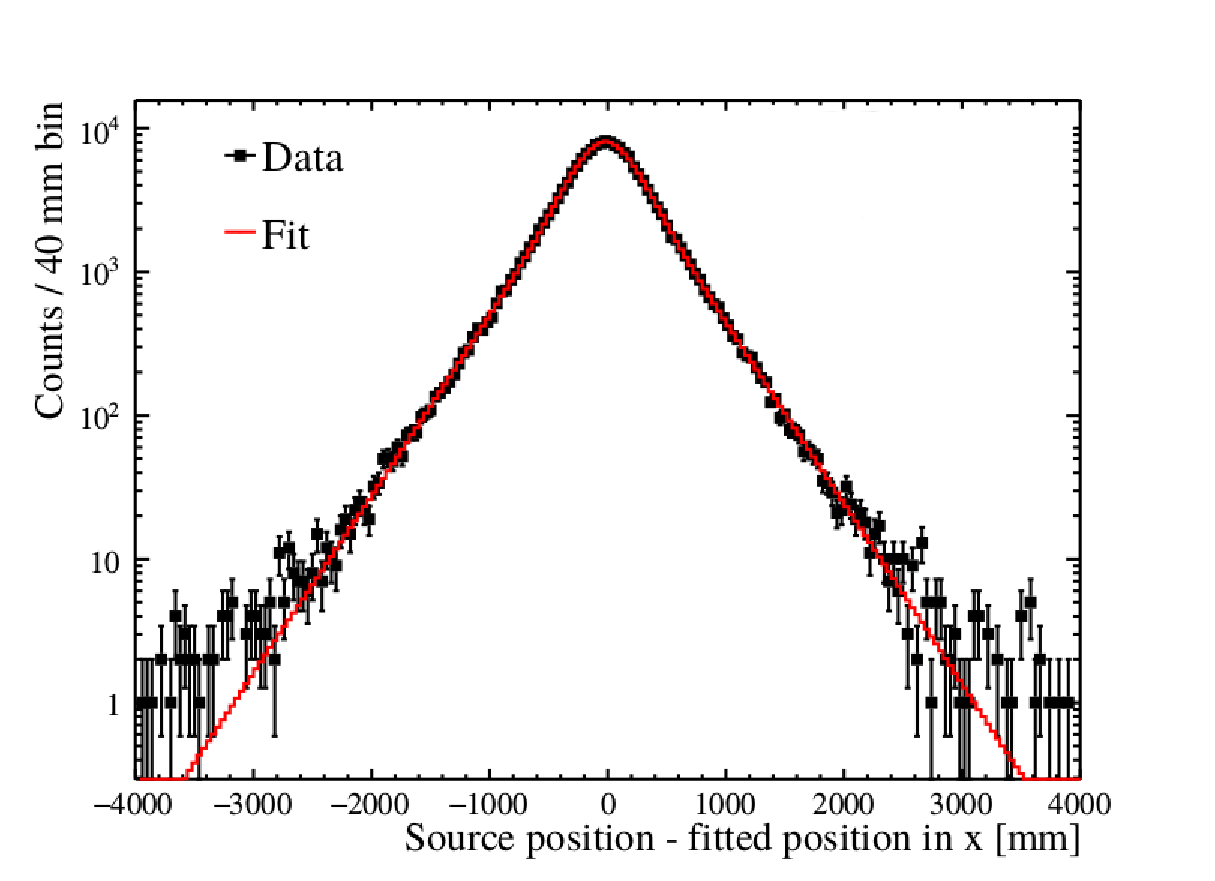
\includegraphics[width=\textwidth]{n16_position_fit_example}
        \caption{}
    \end{subfigure}
\caption[Reconstructed Postion for $\ce{^{16}N}$ events, Data and MC]{
    (a) Reconstructed position of $\ce{^{16}N}$ detected events and MC simulated
    events for a central $\ce{^{16}N}$ run. (b) An example fit to detected events,
    also for a central $\ce{^{16}N}$ run.}
\label{fig:n16_position_comparison}
\end{figure}

With this model three types of position uncertainties are considered, a shift
uncertainty, a resolution uncertainty, and a scale uncertainty.
Here a position shift is the value for $\mu$ in equation~\eqref{eqn:n16_position_model}
averaged over the entire detector volume, $\langle \mu \rangle$;
the position shift systematic then is the difference in $\langle \mu \rangle$
from MC simulation and as determined by detector data.
Rather than averaging over all source positions $\langle \mu \rangle$
is determined averaging over scans along the $x$, $y$ and $z$ axis and
so a position shift for each axial direction is determined.
Only source positions along each axis are used to avoid possible correlations
in each direction's position shift. The resulting systematic uncertainties along
each axial direction are given in table~\ref{tbl:position_shift_systs}.
\begin{table}
    \centering
    \begin{tabular}{|c|c|}
            \hline
            &$\langle \mu \rangle$ Systematic Uncertainty (mm)\\
            \hline
            x&+16.4, -18.2\\
            y&+22.3, -19.2\\
            z&+38.4, -16.7\\
            \hline
    \end{tabular}
    \caption{Position shift systematic uncertainties}
    \label{tbl:position_shift_systs}
\end{table}

The position resolution systematics is evaluated in a similar way as the position
shift systematic, comparing values for
$\sigma^{2}$ in equation~\eqref{eqn:n16_position_model} instead of $\mu$,
but otherwise following the same procedure.
Table~\ref{tbl:position_resolution_systs} gives the extracted position resolution systematics uncertainties
in $\text{mm}$. The uncertainties are given as one-sided because a resolution uncertainty,
unlike the shift uncertainty,
can only be applied to MC simulation by applying addition smearing.
\begin{table}
    \centering
    \begin{tabular}{|c|c|}
            \hline
            &$\langle \sigma \rangle$ Systematic Uncertainty (mm)\\
            \hline
            x&104.0\\
            y&98.2\\
            z&106.2\\
            \hline
    \end{tabular}
    \caption{Position resolution systematic uncertainties}
    \label{tbl:position_resolution_systs}
\end{table}


The final position systematic considered is the position scale uncertainty,
which represents any position dependent shift in $\mu$ between simulation
and data. Unlike the previous two uncertainties this systematic can effect the
number of events that would be predicted to fall within a volume if the
events are distributed uniformly throughout space. For this reason the position
scale systematic is sometimes called the fiducial volume systematic.

The position scale for simulation and data is determined by fitting the values
of $\mu$ as a function of position, along each axis, with a linear function.
The best fit slope for that line gives the position dependence of the position
shift. The value for that shift is defined to be zero at the center
of the detector. The position scale systematic can be though of as the
positional divergence introduced by the MC simulation compared to the detector
data. Table~\ref{tbl:position_scale_systs} gives the position scale systematic
uncertainty along each axis.

\begin{table}
    \centering
    \begin{tabular}{|c|c|}
            \hline
            &Position Scale Systematic Uncertainty (\%)\\
            \hline
            x&+0.91, -1.01\\
            y&+0.92, -1.02\\
            z&+0.91, -0.99\\
            \hline
    \end{tabular}
    \caption{Position scale systematic uncertainties}
    \label{tbl:position_scale_systs}
\end{table}

These uncertainties, the position shift, scale, and resolution are applied
by modifying the positions of simulated events.
For the shift uncertainty the shift uncertainties are simply added to the reconstructed
position.
In general the shift uncertainty has no effect at all on the final result because
just as many events will be shifted into the fiducial volume as are shifted out.

For the resolution a three-dimensional Gaussian centered at the reconstructed
position is created,
with uncorrelated widths given by the position resolution uncertainty along each axis.
From that Gaussian 1000 samples are drawn, and the fraction of those samples
that fall within the fiducial volume is taken to be the weight
that event adds to the histogram for this systematic.
Similar to the position shift uncertainty, the position resolution uncertainty
tends to bring as many events into the fiducial volume as it brings out.
So the position resolution systematic has a negligible effect on the final result.

The position scale systematic shifts the simulated event postions by
\begin{equation}
    \vec{p}\,^{\prime} = (1+\vec{scale})\vec{p}\text{,}
\end{equation}
where the vector $\vec{scale}$ is the postion scale systematic uncertainties.
The fiducial volume cut is applied to the scaled position to generate a
systematically modified histogram.

\subsection{Direction}
\label{sec:angular_systematics}
\begin{figure}[htbp]
    \centering
    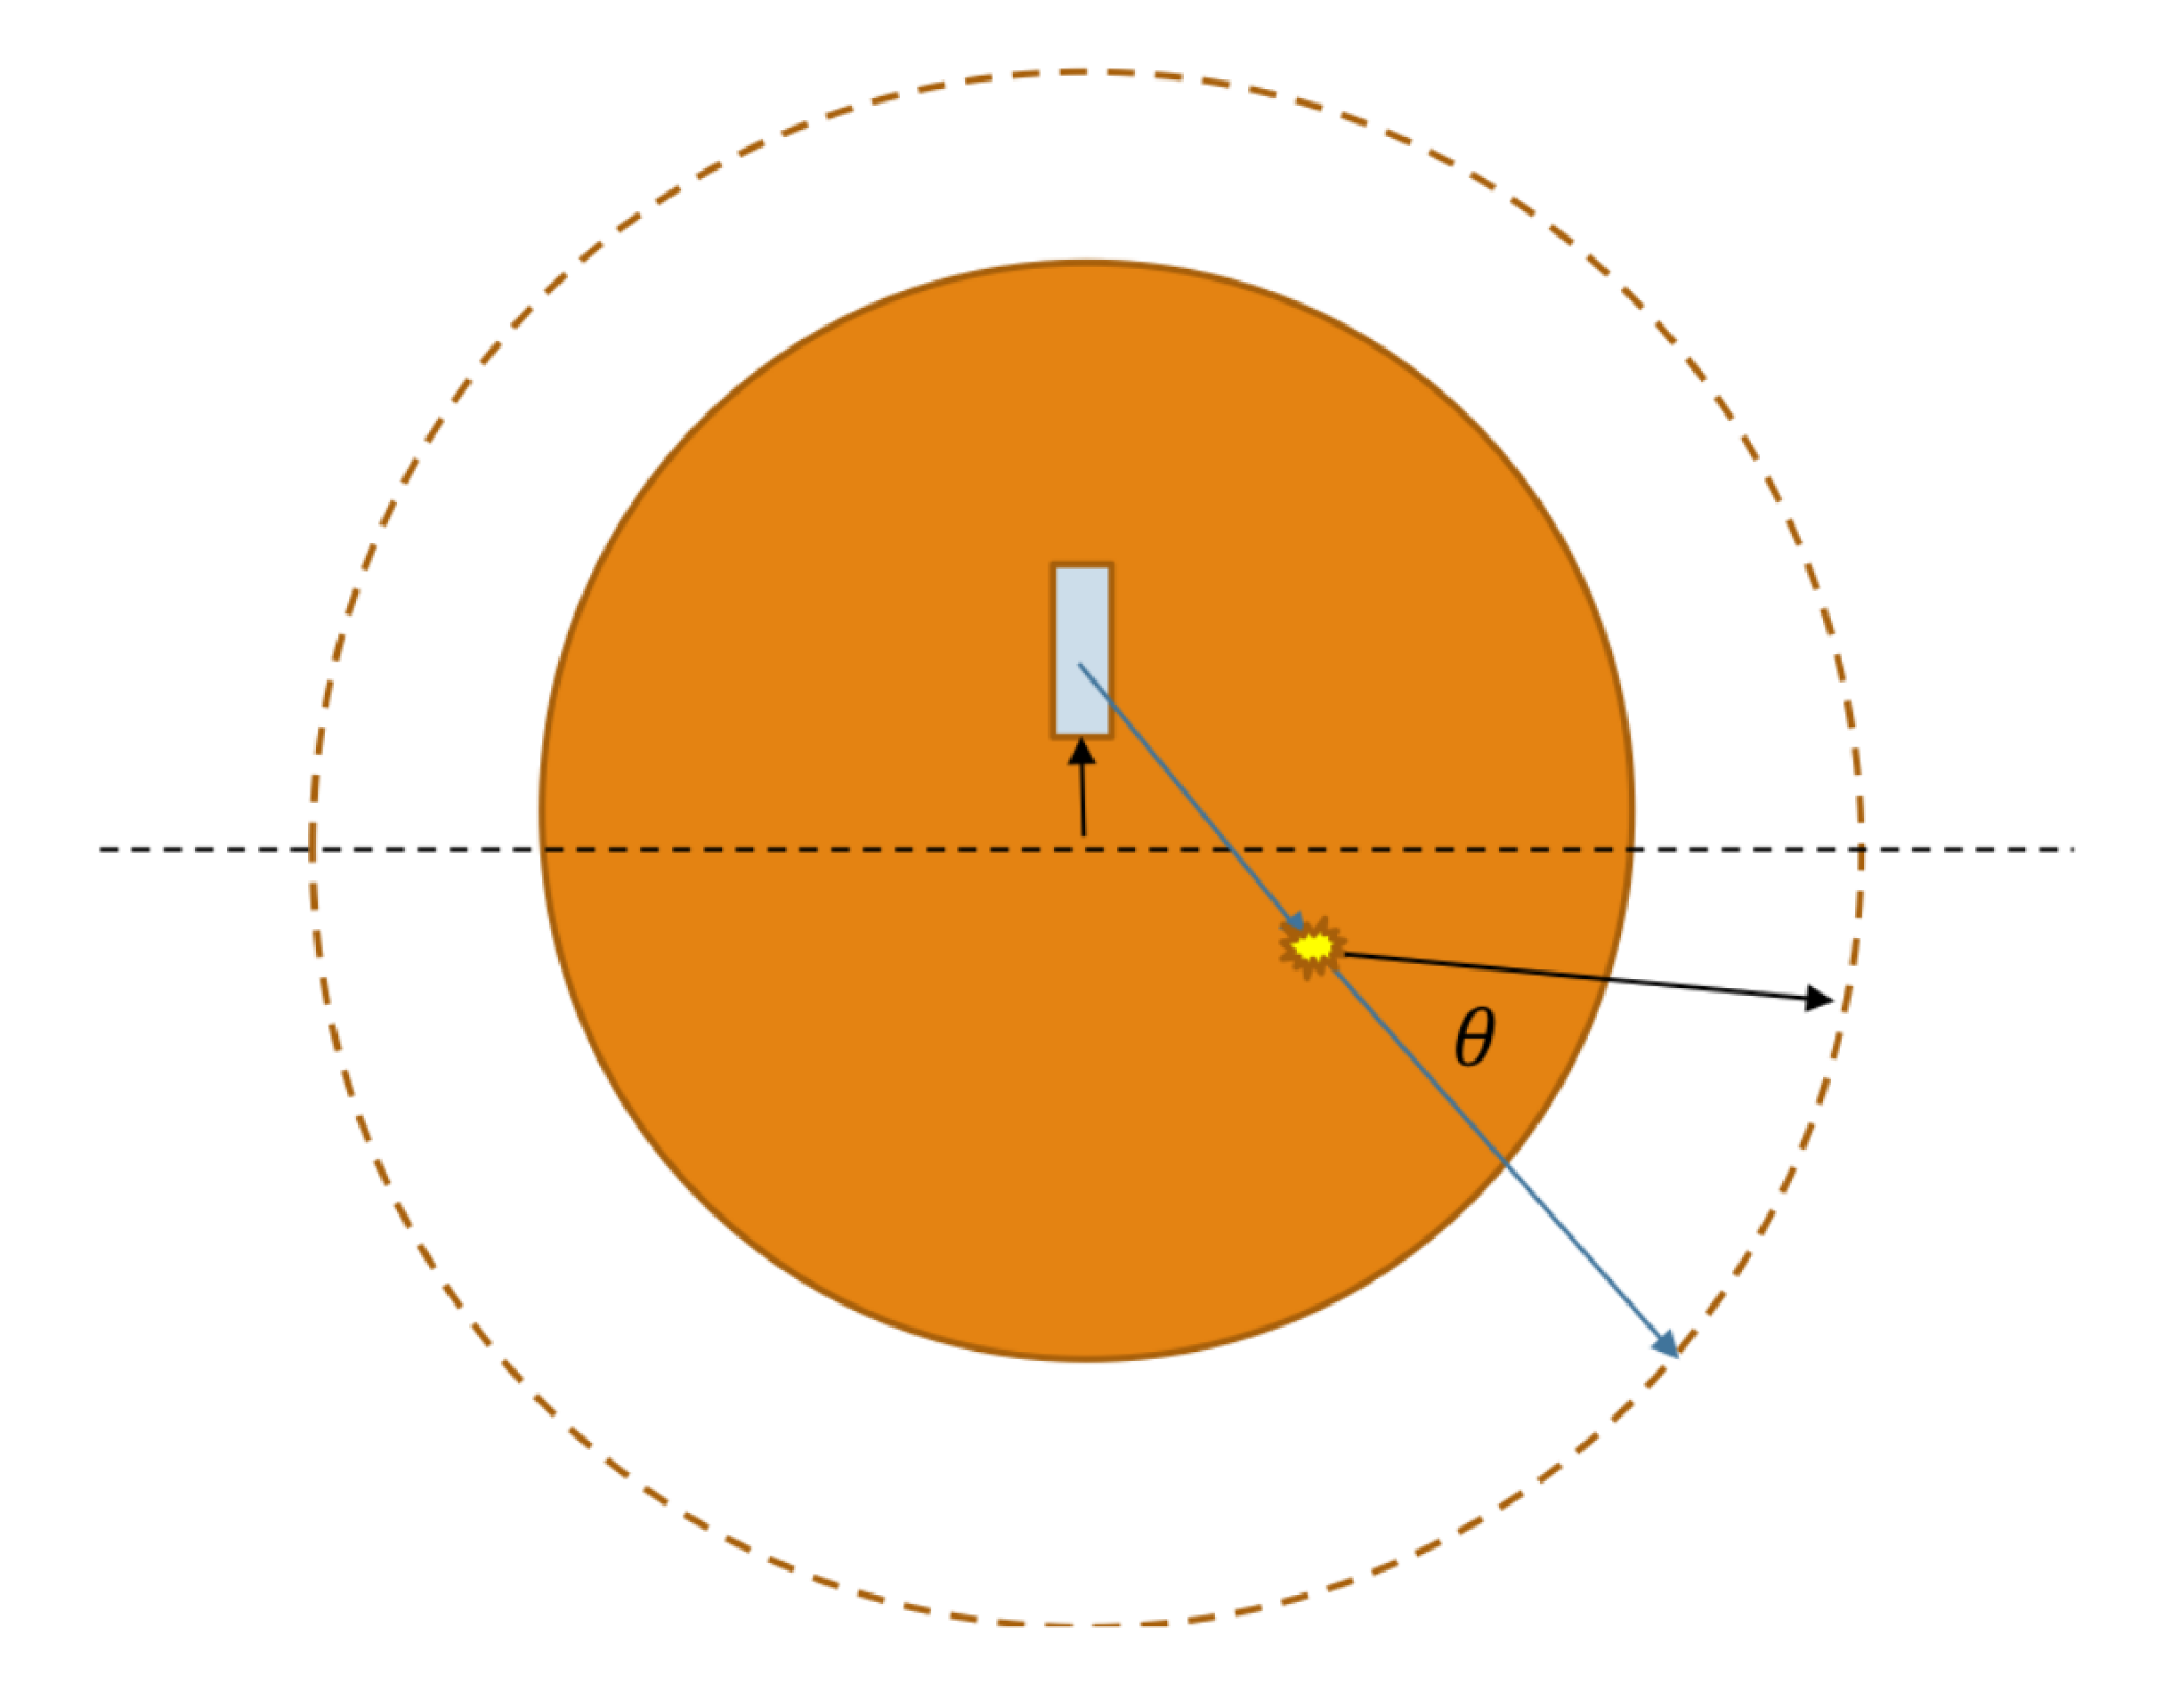
\includegraphics[width=0.72\textwidth]{direction_n16_cartoon}
    \caption[Cartoon of Direction Reconstruction With $\ce{^{16}N}$]{
        Cartoon depicting ``true'' angle reconstruction with $\ce{^{16}N}$
    source. The blue direction is the formed by reconstructed position
of the interaction and the known position of the source. That direction
    is compared to the reconstructed direction (black arrow).}
    \label{fig:n16_direction_cartoon}
\end{figure}
Like position and energy, the direction reconstruction systematics are
determined using data from the $\ce{^{16}N}$ source.
For each $\ce{^{16}N}$ event the direction
of the gamma is estimated as co-linear with the vector from the source
position to the reconstructed event position. The dot product of that vector
with the reconstructed event direction is taken, this gives the value $\cos\theta$
for that event,
\begin{equation}
    \cos\theta = \frac{\vec{p}_{\mathrm{fit}} - \vec{p}_{\mathrm{source}}}
                {\abs{\vec{p}_{\mathrm{fit}} - \vec{p}_{\mathrm{source}}}} \cdot \vec{d}_{\mathrm{fit}}\text{.}
\end{equation}
Figure~\ref{fig:n16_direction_cartoon} schematically shows how $\cos\theta$ is
determined.

A fit is then performed to the distribution of events in $\cos\theta$ using
the model of a double exponential,
\begin{equation}
    P(\cos\theta) = \alpha\beta_{s}\frac{e^{\beta_{s}(\cos\theta -1)}}{1-e^{-\beta_{s}}} +
                    (1-\alpha)\beta_{l}\frac{e^{\beta_{l}(\cos\theta - 1)}}{1-e^{-\beta_{l}}}\text{.}
    \label{eqn:direction_model}
\end{equation}
Where $\beta_{s}$ and $\beta_{l}$ represent the ``short'' and ``long'' decay constants
for the two exponentials, and $\alpha$ represents the relative
strength of the short exponential vs the long one.
This model was developed by the SNO experiment~\citep{scott_oser_direction},
the two decay constants represent the single and multiple-scattering
contributions.
Here Eqn.~\eqref{eqn:direction_model} is used here simply as an empirical
method to parameterize the distribution of events in $\cos\theta$.
Figure~\ref{fig:n16_direction} shows a comparison between data and Monte Carlo
for a central $\ce{^{16}N}$ run and an example fit to the data.
\begin{figure}[htbp]
    \centering
    \begin{subfigure}{0.48\textwidth}
    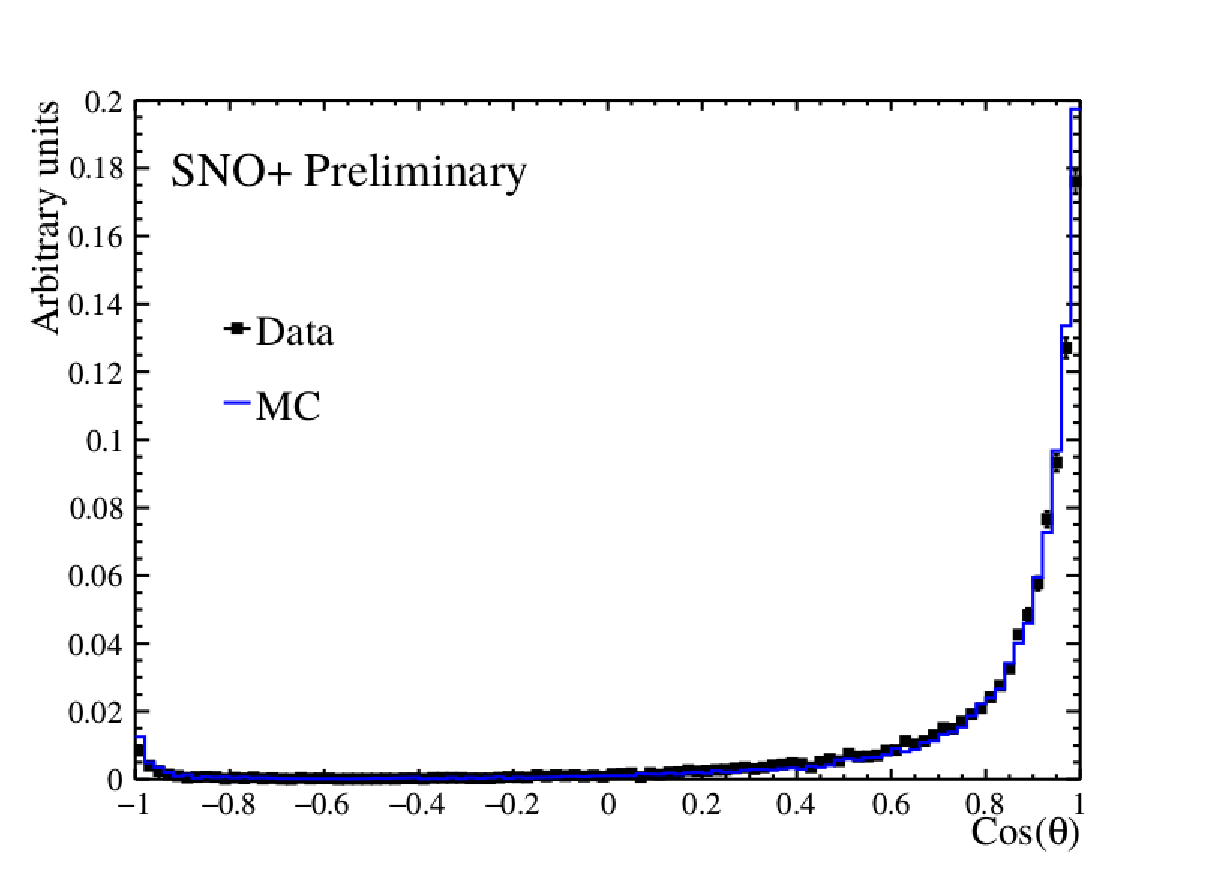
\includegraphics[width=\textwidth]{Direction_data_vs_mc_linear}
    \caption[]{}
    \end{subfigure}
    \hfill
    \begin{subfigure}{0.48\textwidth}
    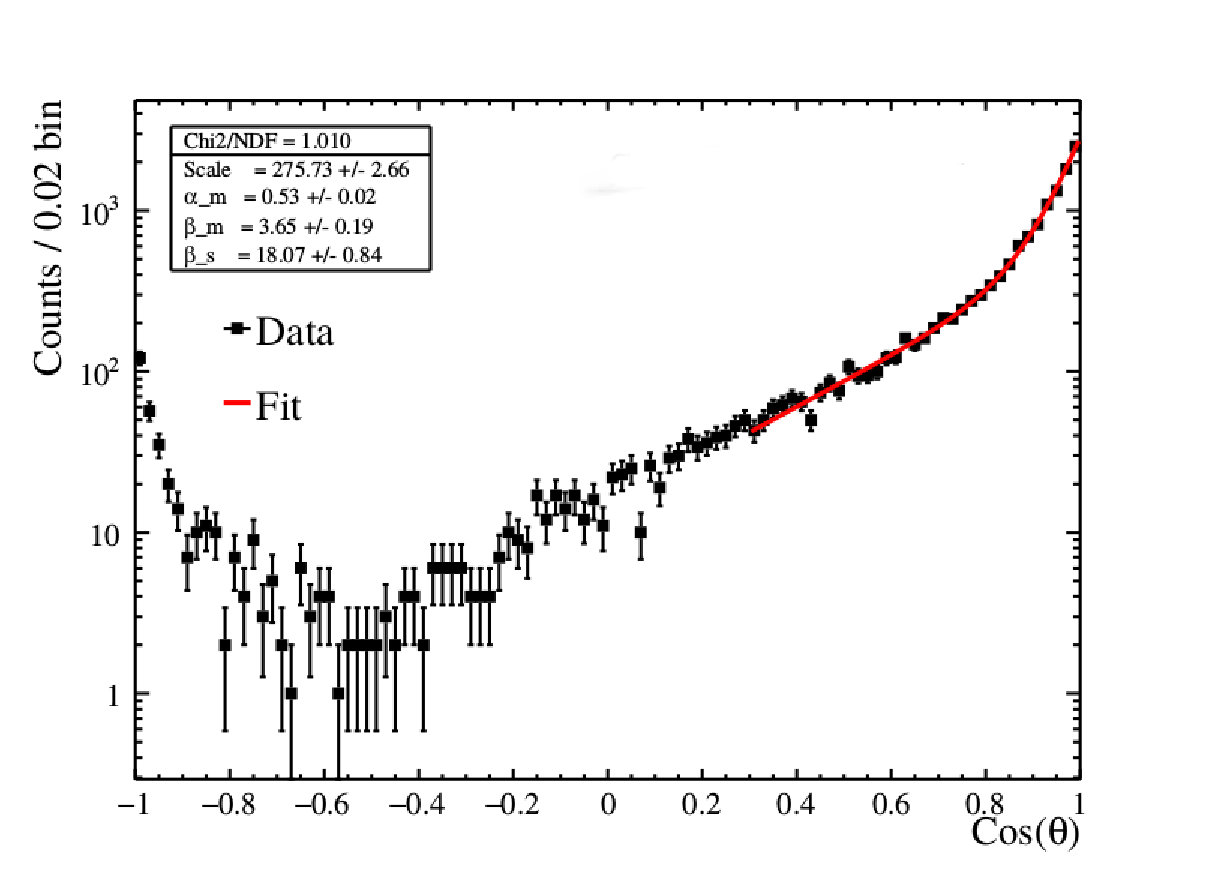
\includegraphics[width=\textwidth]{Direction_fit}
    \end{subfigure}
        \caption[$\ce{^{16}N}$ Direction Reconstruction Comparison]{(a) The
        comparison between data and Monte Carlo simulation for a central
        $\ce{^{16}N}$ run. (b) The fit of Eqn.~\eqref{eqn:direction_model}
        to data for a central $\ce{^{16}N}$ run.}
\label{fig:n16_direction}
\end{figure}
\begin{table}
    \centering
    \begin{tabular}{p{7cm}|p{2cm}|p{2cm}}
        \hline
        Parameter & $\mu$ [\%] &  $\sigma$ [\%] \\
        \hline
        \hline
        $\Delta(\alpha)_{rel} \equiv (\alpha_{data} - \alpha_{MC}) / \alpha_{MC}$  & 7.1 & 10.97 \\
        $\Delta(\beta_s)_{rel} \equiv (\beta_{data} - \beta_{s, MC}) / \alpha_{MC}$     & -6.9 & 11.6 \\
        $\Delta(\beta_l)_{rel} \equiv (\beta_{l, data} - \beta_{l, MC}) / \beta_{S, MC}$      & -2.9 & 10.4 \\
        \hline
    \end{tabular}
    \caption[Relative Uncertainties for Direction Reconstruction]{The
    relative difference in best fit values of Eqn~\eqref{eqn:direction_model}
    from $\ce{^{16}N}$ data and simulation. Here $\mu$ represents the
    best fit value and $\sigma$ is the uncertainty on that value.}
    \label{tbl:direction_recon}
\end{table}
It is shown in~\citep{pierre_luc_thesis} that the systematic uncertainties on the
parameters derived from~\eqref{eqn:direction_model} can be transformed to a shift
in $\cos\theta$ given by,
\begin{equation}
    \cos\theta^{\prime} = 1+(\cos\theta-1)(1+\delta_{\theta})\text{,}
    \label{eqn:direction_shift}
\end{equation}
where $\delta_{\theta}$ is the relative systematic uncertainty of $\beta_{s}$ and $\beta_{l}$.
These relative uncertainties are given in Tbl.~\ref{tbl:direction_recon}.
Transformed this way the systematic uncertainty for the direction reconstruction
is given by
\begin{equation*}
    \delta_{\theta} = +0.08\text{,} -0.13\text{,}
\end{equation*}
the full derivation of these uncertainties can be found in Ref~\citep{snop_water_unidoc}.

The angular resolution uncertainty is propagated to the final result
differently from the other
uncertainties because the distribution of events in $\cos\theta_{sun}$ is
directly related to the direction resolution.  To minimize the impact the
angular resolution has on the result it is used as one of the parameters in the
fit to the $\cos\theta_{sun}$ solar neutrino distribution, and constrained by
the results of the $\ce{^{16}N}$ analysis.

The angular resolution systematic is applied using Eqn.~\eqref{eqn:direction_shift}.
Where $\theta$ is the angle between the true event direction and the reconstructed
event direction, and $delta$ is the angular resolution systematic uncertainty.
Using Eqn.~\eqref{eqn:direction_shift} has the unfortunate downside producing
unphysical values for $\cos\theta^{\prime}$ for values of $\cos\theta\approx-1$.
For values of $\cos\theta^{\prime}$ below $-1$ the value is instead replaced
with a random value drawn from a uniform distribution $\left[-1\text{, }1\right]$.
The logic behind this choice is that when an event reconstructs with a direction
that's nearly $180^{\circ}$ from the correct value, then the reconstruction
has likely failed to such a degree that the reconstructed values are uncorrelated
with the true values, and so drawing from a uniform random distribution preserves
that uncorrelated nature without adding any additional bias.

Once the systematically varied value for $\cos\theta$ is determined, the new angle
needs to be transformed into a corresponding direction vector for the particle.
To do this first a vector that is normal to the plane spanned by the reconstructed
and true direction vector is found by taking the cross-product between those vectors,
\begin{equation}
    \vec{d}_{\mathrm{norm}} = \vec{d}_{\mathrm{true}} \cross \vec{d}_{\mathrm{recon}}\text{.}
\end{equation}
Then $\vec{d}_{\mathrm{recon}}$ is rotated around $\vec{d}_{\mathrm{norm}}$
such that the rotated vector $\vec{d}^{\prime}_{\mathrm{recon}}$ now has an angle
of $\theta^{\prime}$.
The direction $\vec{d}^{\prime}_{\mathrm{recon}}$ is then used in the
analysis to generate event distributions in $\cos\theta_{sun}$.

Following this procedure PDFs for $\cos\theta_{sun}$ are generated for many
values of $\delta_{\theta}$, producing $P(\cos\theta_{sun}, \delta_{\theta})$.
The constraint on $\delta_{\theta}$ produced by the $\ce{^{16}N}$ analysis
are included in this two-dimension PDF\@.
$P(\cos\theta_{sun}, \delta_{\theta})$ is used in the remainder of the analysis
treating $\delta_{\theta}$ as a nuisance parameter.

\subsection{Mixing Parameters}
The central values and uncertainties of the neutrino mixing parameters, $\Delta
m^{2}_{21}$, $\theta_{12}$ and $\theta_{13}$ is taken from Ref.~\citep{pdg_globalfit}.
\begin{table}
    \centering
    \begin{tabular}{c | c | c}
        Parameter & Value & Uncertainty\\
        \hline
        $\Delta m^{2}_{21}$ & $7.37\times10^{-5} \mathrm{MeV}/\mathrm{c}^{2}$ & +0.17, -0.16\\
        $\theta_{12}$ & $33.02^{\circ}$ & 0.537, -0.455 \\
        $\theta_{13}$ & $8.41^{\circ}$ & -- \\
        $\Delta m^{2}_{31}$ & $2.5\times10^{-3}\mathrm{MeV}/\mathrm{c}^{2}$ & -- \\
    \end{tabular}
    \caption{A summary of the mixing parameters and their uncertainties as used in 
    propagation of systematic uncertainties. Values from Ref~\citep{pdg_globalfit}.}
\label{tbl:mixing_values}
\end{table}
The values and uncertainties for the mixing parameters
are summarized in Table~\ref{tbl:mixing_values}.
A survival probability curve is generated for each of the mixing parameters
shifted by their positive and negative one-sigma uncertainty.
These systematically adjusted PDFs are used in the analysis replacing the
standard survival probability curve to propagate the uncertainties to the
flux result.
\subsection{Trigger Efficiency}
The uncertainty on the trigger efficiency is described in Sec~\ref{sec:trigeff}.
PDFs for $\cos\theta_{sun}$ are generated using the more pessimistic
trigger efficiency curves measured by the laserball and TELLIE\@.
Simulated events that have an in-time nhit that is predicted by the nhit-monitor
to be 100\% efficient are de-weighted to match the laserball efficiency
measurement.
The histogram that results from the de-weighted events are used as the systematically
adjusted histogram to account propagate the trigger efficiency uncertainty to the
flux result.
The weight used for each value of $\tilde{n}_{100}$ is given in Tbl.~\ref{tbl:trigg_eff}.

\begin{table}
    \centering
    \begin{tabular}{c| c}
        $\tilde{n}_{100}$ & High Trigger Period Weight\\
        \hline
        24 & 0.983\% \\
        25 & 0.991\%\\
        26 & 0.997\%\\
        \end{tabular}
        \caption[Solar Analysis Trigger Efficiecy Systmatics]{
            Weight given to events with values for $\tilde{n}_{100}$ above
            cut value for the high threshold period, but where the nhit-monitor and laserball disagree.}
        \label{tbl:trigg_eff}
\end{table}
